
%%******************************************************************************
%% SECTION - Cronograma 
%%******************************************************************************
\newgeometry{margin=1cm}
\begin{landscape}
\thispagestyle{empty} %% Remove header and footer.

\vspace*{2cm}
\section{Cronograma}
\label{cronograma}

\vfill

\begin{center}
    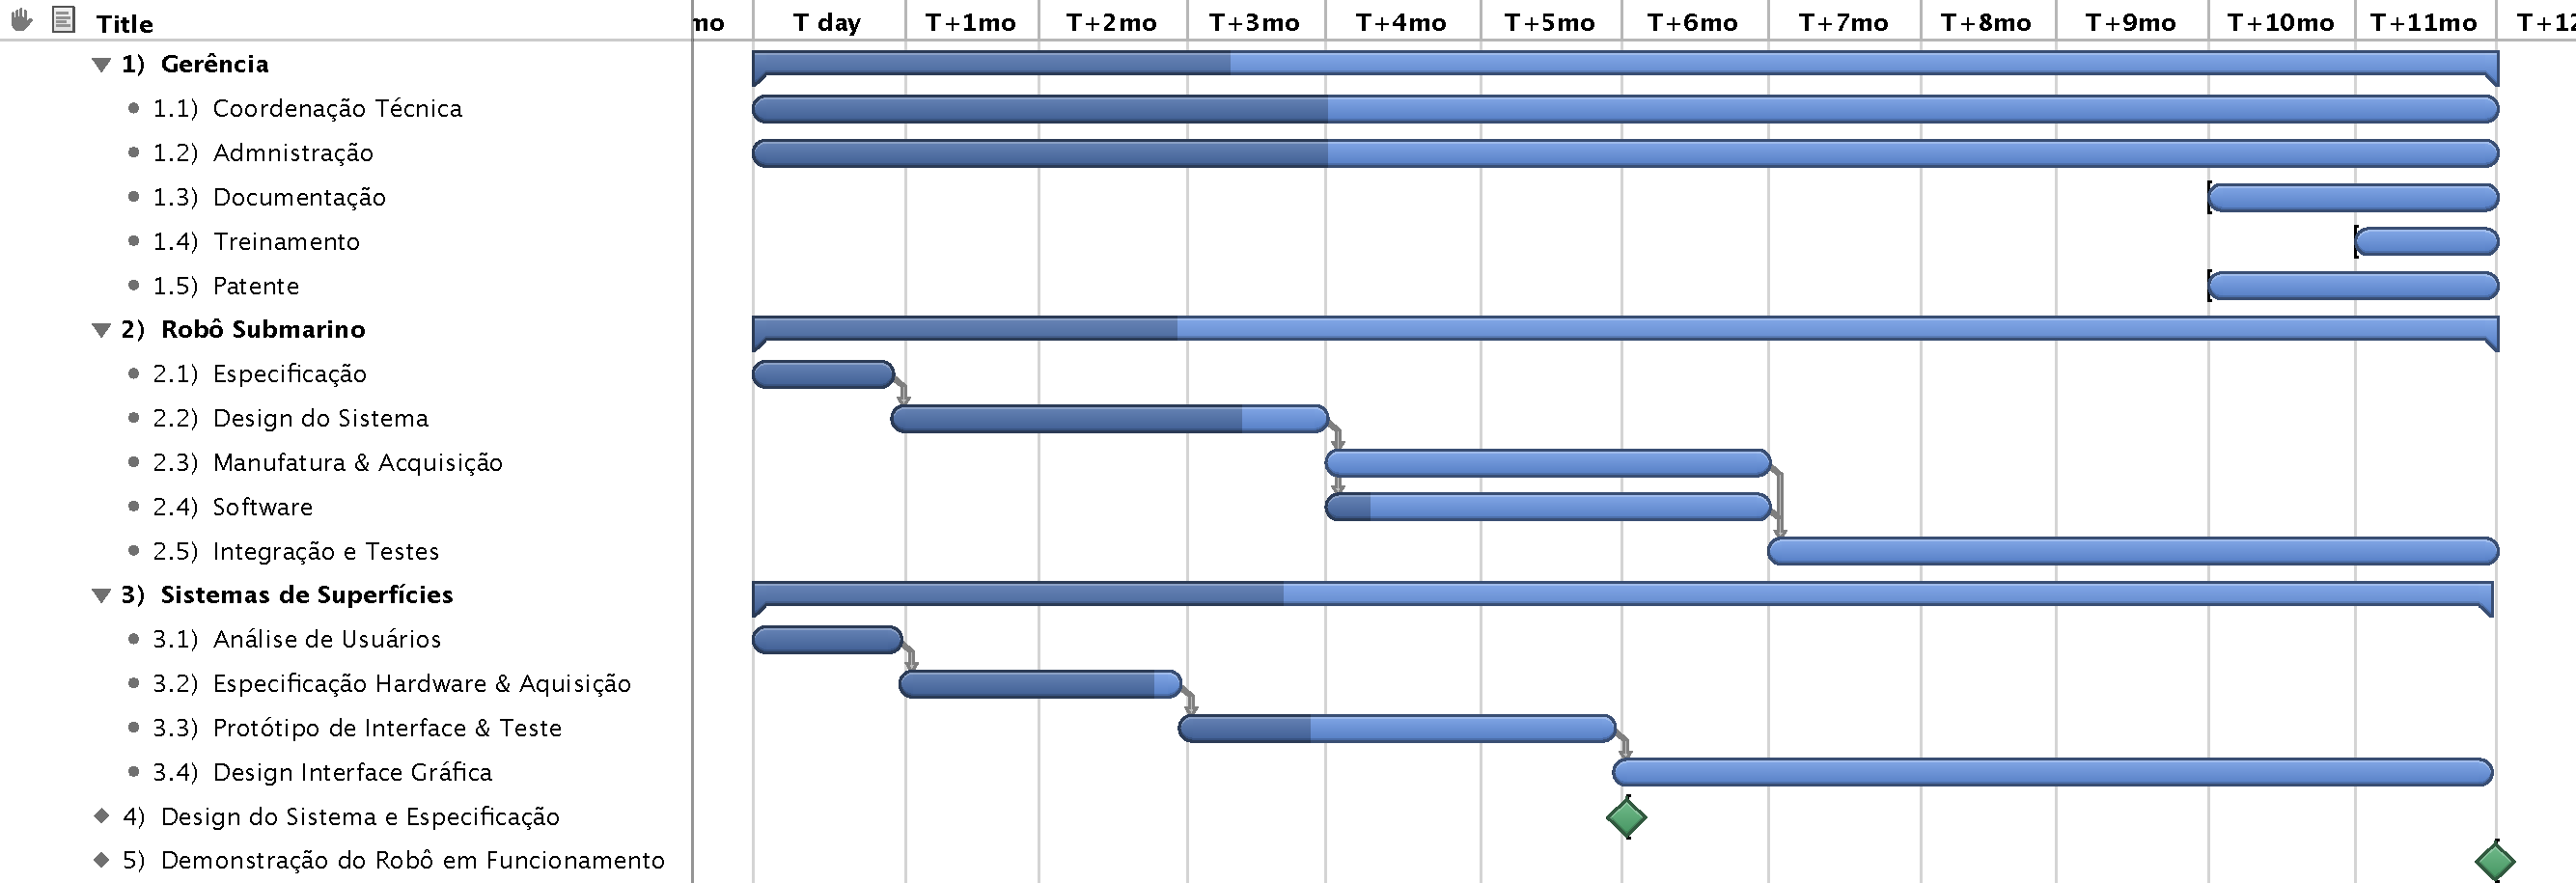
\includegraphics[width=1\columnwidth]{figs/gantt/Gantt.pdf}
\end{center}

\vfill
\vspace*{2cm}
\end{landscape}
\restoregeometry


{\bf  1) Gerência}: O planejamento tecnológico e administrativo, organização, coordenação e controle utilizados para alcançar os objetivos gerais do projeto, que não estão associados a hardware específico ou elementos de software. 

\begin{description}

\item[1.1) Coordenação Técnica]: Coordenar a parte técnica do projeto, atribuindo tarefas e revendo o trabalho concluído. O resultado da coordenação técnica no período e seus entregáveis foram: 

\begin{description}
	\item [Status] - Tarefa em andamento, sem atrasos. 
	\item [Entregável 01] - Atas de reuniões de acompanhamento técnico e alocamento de tarefas.  
	\item [Entregável 02] - Relatório Mensais 01, 02 e 03. 
	\item [Entregável 03] - Relatório Quadrimestral 01. 
\end{description} 


\item[1.2) Administração]:  Administrar a parte financeira do projeto. O resultado são as planilhas do balanço financeiro do projeto atualizada 

\begin{description}
	\item [Status] - Tarefa em andamento, sem atrasos.  
	\item [Entregável 01] - Relatório Mensais 01, 02 e 03. 
	\item [Entregável 02] - Relatório Quadrimestral 01. 
\end{description} 


	\item[1,3) Documentação:] este pacote de trabalho lida com a escrita da documentação técnica e de operações. Os resultados são os manuais e a documentação técnica do sistema.

\begin{description}
	\item [Status] - Tarefa não iniciada. 
\end{description} 

	\item[1,4) Treinamento:] esforço necessário para treinar o pessoal de operação da hidrelétricas no uso do  sistema robótico desenvolvido no projeto.

\begin{description}
	\item [Status] - Tarefa não iniciada. 
\end{description} 

	\item[1,5) Patente:] solicitação de patente de produto para o sistema robótico desenvolvido.

\begin{description}
	\item [Status] - Tarefa não iniciada. 
\end{description} 

\end{description}


\begin{description}

\vspace{0,5cm}

\item[ 2)  Robô Submarino:] este elemento lida com o trabalho necessário para desenvolver o sistema eletromecânico do robô. 

\item[2,1) Especificação:] neste pacote de trabalho, requisitos do sistema serão especificados através de reuniões com os funcionários responsáveis pela operação na hidroelétrica e através de observações em campo. O resultado será um documento com os requisitos do sistema.

\begin{description}
	\item [Status] - Tarefa Concluída. 
	\item [Entregável 01] - Documento de Projeto Básico. 
\end{description} 

\item[2,2) Design do Sistema:] processo de definição da arquitetura, componentes, módulos e interface que satisfazem os requisitos do sistema. O resultado será uma lista de componentes, arquitetura de software e design eletromecânicos do sistema.

\begin{description}
	\item [Status] - Tarefa em Andamento, atraso de de 1 mês. A lista de componentes e design elétrico pevistor para este pacote de trabalho foram concluídos e estão detalhados no documento de Projeto Básico. Entretanto, dado os atrasos de pagamento das parcelas do projeto não foi possível contratar os serviços de design mecânico e de software. 
\end{description} 

\item[2,3) Manufatura e Aquisição:] compra e construção dos componentes definidos durante a fase de design do sistema. O resultado serão as partes que integradas formarão o robô. 

\begin{description}
	\item [Status] - Tarefa não iniciada. 
\end{description} 

\item[2,4) Software:] desenvolvimento de drivers, controladores e comunicação para o hardware do robô. O resultado será uma biblioteca de componentes  do software.

\begin{description}
	\item [Status] - Tarefa iniciada.
\end{description} 

\item[2,5) – Integração e Teste:] os componentes eletrônicos, mecânicos e de software serão integrado no sistema Viga Pescadora Inteligente. Este pacote de trabalho também inclui a instalação e teste do sistema.

\begin{description}
	\item [Status] - Tarefa não iniciada. 
\end{description} 

\end{description}


\begin{description}

\vspace{0,5cm}

\item[3) Sistemas de Superfície] Este elemento inclui o hardware e o software necessários para a operação do robô na superfície, incluindo a concepção, desenvolvimento, implementação e integração da comunicação, interface e gerência de dados. 

\item[3,1) Análise de Usuário:] Análise dos potenciais usuário do sistemas. Este pacote de trabalho vai resultar em um documento que define: O que o usuário espera do sistema. Como o sistema irá fazer parte do dia a dia da operação. Qual é a capacitação técnica do futuro usuário. Qual aparência de interface têm um maior apelo para o usuário.

\begin{description}
	\item [Status] - Tarefa Concluída. 
	\item [Entregável 01] - Documento de Análise de Usuário.
\end{description} 

\item[3,2) Especificação de Hardware e Aquisição] este pacote de trabalho inclui a especificação e aquisição do equipamento necessário para operar o robô a partir da superfície. O resultado é um lista de componentes e respectivos fabricantes a serem comprados para o projeto. 

\begin{description}
	\item [Status] - Tarefa Atrasada, 1 mês. O equipamento foi especificado entretanto devido ao atraso do pagamento das parcelas do projeto a aquisição não foi realizada. 
\end{description} 


\item[3,3) Protótipo de Interface e Teste] desenvolvimento de telas interativas simples, sem conteúdo, concentrando apenas no desenvolvimento da parte visual da interface. Estes protótipo de interface vai ser testado com os futuros usuário dos sistema e o resultado da sensação da mesma será avaliada.

\begin{description}
	\item [Status] - Tarefa iniciada. 
\end{description} 

\item[3,4) Interface de Usuário] implementação da interface de usuário (GUI) do robô, o que permite a visualização e o seu controle. O resultado será um software. 

\begin{description}
	\item [Status] - Tarefa não iniciada. 
\end{description} 


\end{description}